\section{Naive Bayes}
Assume all features are independent effects of the label. This means that for $n$ features, \\
$P(Y,F_1,...,F_n)=P(Y)\Pi_{i}P(F_{i}|Y)$ \\
\begin{figure}[H]
\centering
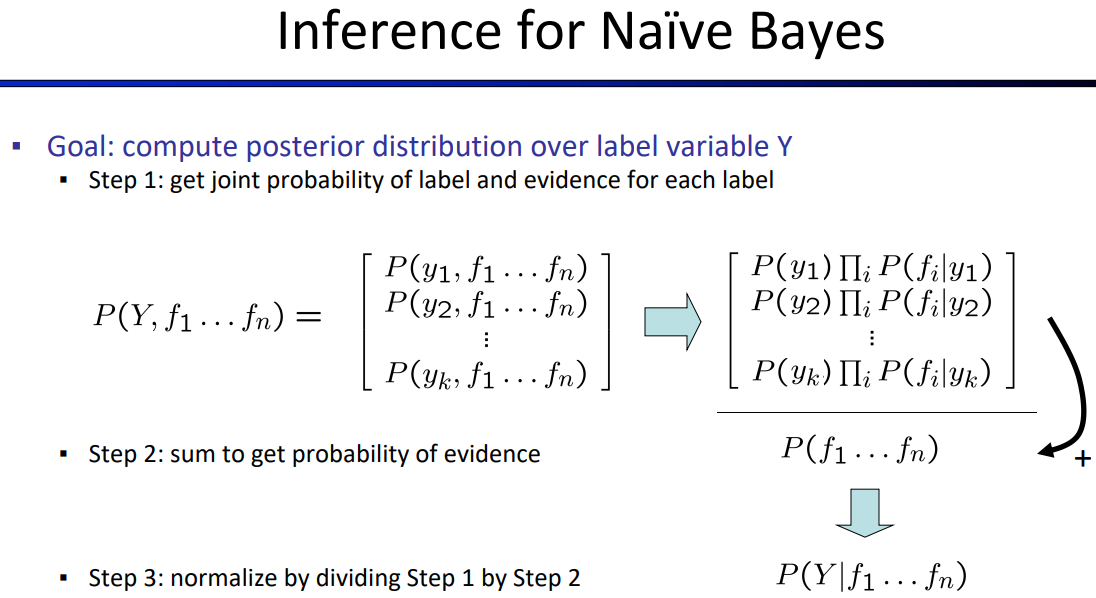
\includegraphics[width=\linewidth]{naive-bayes-inference}
\end{figure}
To compute these, we need the prior over labels $P(Y)$ and $P(F_{i}|Y)$ for each feature. These parameters are calculated from training data counts. Make sure to split data into training, validation (held-out), and testing data. Overfitting is when model too closely fits training data and can't generalize, so we can \textbf{smooth} or \textbf{regularize} the estimates. We can do \\
\textbf{Laplace Smoothing}: Pretend you saw each outcome $k$ extra times; higher $k$ means more smoothing, closer to a uniform distribution. We want to tune $k$ and other hyperparameters on the validation or held-out data.